\chapter{Gestión de proyecto software}
\label{Gestión de proyecto software}

Este capítulo simula la gestión del proyecto en las condiciones habituales de un entorno
empresarial, tal como exige la titulación. No describe, por tanto, la forma en que se ha gestionado
el Trabajo de Fin de Máster —eso se recoge en el anexo
\ref{Seguimiento de proyecto fin de máster}—, sino cómo se habría planificado, presupuestado y
controlado el mismo desarrollo si lo hubiera acometido una empresa de ingeniería para un cliente
del sector del petróleo y el gas.

El supuesto de partida es el siguiente: una empresa de servicios de automatización recibe el
encargo de evaluar la viabilidad de automatizar el accionamiento de válvulas de volante mediante un
robot humanoide, y de entregar un dictamen fundamentado sobre qué familia de algoritmos de
aprendizaje conviene adoptar antes de invertir en la fase de despliegue. Para que la simulación
tenga fundamento, las duraciones, los recursos y los riesgos se han tomado del desarrollo real; las
tarifas y los precios son estimaciones razonables a fecha de 2026, no ofertas.


\section{Alcance del proyecto}
\label{Alcance del proyecto}

\subsection{Definición del proyecto}

El objetivo del encargo es responder a una pregunta de decisión —¿modelo fundacional o política
específica?— con evidencia experimental obtenida en simulación, antes de comprometer inversión en
hardware y en integración. El cliente no compra un robot que abre válvulas; compra el criterio para
elegir cómo construirlo.

Los entregables comprometidos son cuatro:

\begin{enumerate}
	\item Un \textbf{entorno de simulación} reproducible de la tarea, con el robot y una válvula
	procedente de un modelo CAD del cliente, instrumentado con un criterio de éxito automático.
	\item Un \textbf{conjunto de demostraciones} teleoperadas, documentado y en un formato que sirva
	a ambas familias de métodos.
	\item Un \textbf{banco de evaluación} que enfrente a las políticas a condiciones idénticas y
	produzca las métricas acordadas.
	\item El \textbf{dictamen}: la comparación cuantitativa, su análisis estadístico y la
	recomendación, en forma de informe técnico.
\end{enumerate}

Los criterios de aceptación son verificables: el entorno se acepta cuando una demostración
teleoperada abre la válvula y queda grabada con imagen; el conjunto de datos, cuando supera la
verificación de formato y alimenta ambos entrenamientos sin transformación adicional; el banco,
cuando dos políticas distintas se evalúan con el mismo comando y las mismas semillas; y el dictamen,
cuando cada afirmación va acompañada de su intervalo de confianza y su contraste.

Queda \textbf{fuera de alcance}, y así se hace constar en la oferta: el despliegue sobre robot
físico, la certificación del sistema para zona ATEX, la integración con el sistema de control de la
planta, y cualquier tarea distinta de la apertura de válvulas de volante. Cada una de esas cuatro
cosas es un proyecto por sí misma, y el dictamen debe precisamente decir si merece la pena acometer
la primera.

\subsection{Estimación de tareas y recursos}

El trabajo se descompone en cinco paquetes, más uno transversal de gestión, y cada paquete se asigna
al perfil que lo lidera:

\begin{description}
	\item[PT1 — Entorno de simulación.] Construcción de la tarea sobre el marco de simulación:
	robot, válvula, criterio de éxito, aleatorización, teleoperación en realidad mixta y grabación.
	Ingeniero de robótica sénior. Es el paquete de mayor incertidumbre, porque integra una pila
	de realidad mixta cuyo comportamiento no se conoce hasta que se monta.
	\item[PT2 — Captura de demostraciones.] Sesiones de teleoperación, verificación de cada sesión
	y aplicación del fondo fotorrealista. Técnico de teleoperación, con apoyo del sénior.
	\item[PT3 — \textit{Pipeline} de datos y entrenamiento.] Conversión al formato común, un
	entorno de ejecución por método y los dos entrenamientos. Ingeniero de aprendizaje automático.
	\item[PT4 — Evaluación y análisis.] Banco de evaluación, tiradas, análisis estadístico y
	figuras. Ingeniero de pruebas, con el de aprendizaje automático.
	\item[PT5 — Documentación y dictamen.] Informe técnico, documentación de lanzamiento y
	entrega del repositorio. Ingeniero de robótica sénior.
	\item[Gestión y seguimiento.] Planificación, reuniones con el cliente, control de riesgos.
	Jefe de proyecto, a tiempo parcial durante todo el proyecto.
\end{description}

La estimación de esfuerzo se ha hecho por analogía con el desarrollo real, redondeada al alza para
absorber la incertidumbre de PT1, y suma \textbf{800 horas} repartidas en dieciséis semanas. La
tabla \ref{tab:presupuesto-personal} la desglosa por perfil.

\subsection{Presupuesto}

A continuación se detalla un presupuesto estimado para el coste total del proyecto. Las tarifas
por hora son coste para la empresa —salario, cargas sociales y estructura— y no tarifas de venta.

\subsubsection{Coste de personal}

\begin{table*}[ht]
	\centering
	\caption{Presupuesto de personal}
	\label{tab:presupuesto-personal}
	\makebox[\textwidth]{
		\begin{tabular}{|l|l|c|c|c|}
			\cline{1-5}
			Tarea &	Perfil & Horas & Euros/Hora  &  Total\\ \hline
			Entorno de simulación & Ingeniero de Robótica Senior & 200 & 100 & 20000 \euro\\
			Captura de demostraciones & Técnico de Teleoperación & 120 & 60 & 7200 \euro\\
			\textit{Pipeline} de datos y entrenamiento & Ingeniero de Aprendizaje Automático & 240 & 100 & 24000 \euro\\
			Evaluación y análisis & Ingeniero de Pruebas & 100 & 80 & 8000 \euro\\
			Documentación y dictamen & Ingeniero de Robótica Senior & 80 & 100 & 8000 \euro\\
			Supervisión del proyecto & Jefe de Proyecto & 60 & 120 & 7200 \euro\\ \hline\hline
			\multicolumn{4}{|c|}{Total} & \multicolumn{1}{c|}{74400 \euro}\\ \hline
		\end{tabular}
	}
\end{table*}

El personal es, con diferencia, la partida dominante: más del 95\,\% del coste antes de impuestos.
Es lo esperable en un proyecto de viabilidad, donde no se compra nada que no exista ya y todo el
valor está en las horas de ingeniería.

\subsubsection{Coste del hardware}

El equipamiento es el que efectivamente se ha empleado en el desarrollo. La tabla
\ref{tab:presupuesto-hardware} recoge su precio de adquisición estimado. Puesto que el equipo sigue
siendo útil después del proyecto, al presupuesto se imputa únicamente su \textbf{amortización}
durante los cuatro meses de duración, con un periodo de amortización lineal de tres años, que es el
habitual para equipos informáticos: 4/36 del precio de compra.

\begin{table*}[ht]
	\centering
	\caption{Equipamiento empleado y coste imputado}
	\label{tab:presupuesto-hardware}
	\makebox[\textwidth]{
		\begin{tabular}{|p{8cm}|c|c|c|}
			\cline{1-4}
			Concepto & Unidades & Precio (Euros) & Imputado (Euros) \\ \hline
			Estación de trabajo PCSpecialist: AMD Ryzen Threadripper 9980X (64 núcleos, 128 hilos), placa Gigabyte TRX50 AERO D, 256\,GB de memoria DDR5, NVMe Corsair MP600 PRO de 4\,TB, chasis, fuente y refrigeración & 1 & 8600 & 956 \\
			GPU NVIDIA RTX PRO 6000 Blackwell Max-Q Workstation Edition, 96\,GB & 2 & 9000 & 2000 \\
			Visor de realidad mixta PICO 4 Ultra, con mandos & 1 & 600 & 67 \\ \hline\hline
			\multicolumn{2}{|c|}{Total} & \multicolumn{1}{c|}{27200} & \multicolumn{1}{c|}{3023} \\ \hline
		\end{tabular}
	}
\end{table*}

Cada pieza tiene una función concreta en el proyecto, y ninguna está sobredimensionada. Las dos
aceleradoras no son un lujo: la teleoperación en realidad mixta necesita una GPU dedicada —la
transmisión al visor no tolera compartirla— y el entrenamiento, la evaluación y la aplicación del
fondo fotorrealista corren en la otra sin interrumpirla; la variante Max-Q, de 300\,W, es lo que
permite alojar dos en una sola estación. Los sesenta y cuatro núcleos del procesador tampoco son
un exceso: la grabación de demostraciones se hace con la física en CPU, porque la combinación de
física en GPU, realidad mixta y cámaras hace fallar al simulador, y con la física en CPU el número
de núcleos es lo que sostiene la tasa de simulación. Los 256\,GB de memoria absorben la
reconstrucción fotorrealista de la escena y el simulador a la vez, y los 4\,TB de almacenamiento
alojan el conjunto de datos —que con el fondo aplicado pesa del orden de 110\,MB por
demostración—, los puntos de control de los modelos y los resultados de cientos de tiradas.

\subsubsection{Coste del software y licencias}

Toda la pila de simulación y de aprendizaje es de uso gratuito o de código abierto: Isaac Sim, Isaac
Lab e Isaac Lab Arena se distribuyen sin coste para desarrollo, CloudXR se obtiene con el registro
de desarrollador de NVIDIA, y LeRobot, los pesos de GR00T, Docker y el sistema operativo son libres.
La única partida de software es la suscripción a herramientas de desarrollo asistido por
inteligencia artificial, cuyo uso se declara al inicio de esta memoria, estimada en 100\,\euro{}
mensuales durante los cuatro meses: \textbf{400\,\euro}.

\subsubsection{Coste total}

El presupuesto incluye una \textbf{contingencia del 10\,\%} sobre el coste directo, que es la forma
habitual de cubrir la materialización de los riesgos de la sección \ref{sec:riesgos} sin renegociar
la oferta; las horas de PT1 ya están redondeadas al alza, pero un proyecto que integra una pila de
realidad mixta por primera vez no debe ofertarse sin margen.

\begin{table*}[ht]
	\centering
	\caption{Presupuesto total}
	\label{tab:presupuesto-total}
	\makebox[\textwidth]{
		\begin{tabular}{|l|r|}
			\cline{1-2}
			Concepto &	Coste (Euros) \\ \hline
			Costes de personal & 74400  \\
			Costes de hardware (amortización) & 3023   \\
			Costes de software y licencias  & 400   \\ \hline
			Coste directo & 77823 \\
			Contingencia (10\,\%) & 7782 \\ \hline
			Subtotal  &  85605 \\
			IVA (21\,\%) & 17977 \\ \hline \hline
			Total Proyecto & \textbf{103582 \euro} \\ \hline
	\end{tabular}}
\end{table*}


\section{Plan de trabajo}
\label{Plan de trabajo}

\subsection{Identificación de tareas}

Los paquetes de trabajo se desglosan en las tareas de la tabla \ref{tab:tareas}, que son las filas
del diagrama de Gantt de la figura \ref{fig:gantt}. Las dependencias son estrictas: cada tarea
consume la salida de la anterior, de modo que no se puede empezar a capturar sin entorno, ni a
entrenar sin datos convertidos, ni a evaluar sin políticas entrenadas.

\begin{table*}[ht]
	\centering
	\caption{Tareas del proyecto y dependencias}
	\label{tab:tareas}
	\makebox[\textwidth]{
		\begin{tabular}{|l|p{6.2cm}|c|l|}
			\cline{1-4}
			Tarea & Contenido & Semanas & Depende de \\ \hline
			T0 Análisis y arranque & Requisitos, activos del cliente, plan & 0--2 & --- \\
			T1 Entorno de simulación & Tarea, robot, válvula, teleoperación, grabación & 1--6 & T0 \\
			T2 \textit{Pipeline} de datos & Conversión, verificación, entornos de ejecución & 4--8 & T1 (parcial) \\
			T3 Captura de demostraciones & Sesiones, verificación, fondo fotorrealista & 7--11 & T1, T2 \\
			T4 Entrenamiento & Ajuste fino y entrenamiento desde cero & 10--13 & T3 (parcial) \\
			T5 Evaluación y análisis & Tiradas, estadística, figuras & 12--15 & T4 \\
			T6 Documentación y dictamen & Informe, documentación, entrega & 13--16 & T5 (parcial) \\
			T7 Gestión y seguimiento & Transversal & 0--16 & --- \\ \hline
		\end{tabular}
	}
\end{table*}

\subsection{Estimación de tareas}

Las duraciones proceden del desarrollo real, con dos ajustes. La primera es que T1 se estima en
seis semanas cuando el núcleo del entorno se levantó en menos: la diferencia es la integración de
la pila de realidad mixta, cuyos fallos no se pueden prever y que en el desarrollo real consumió
sesiones enteras en problemas de configuración sin síntoma visible. Es la tarea de mayor
incertidumbre y la que justifica la contingencia. La segunda es que T3 se estima para un conjunto
de datos de hasta cuatrocientas demostraciones en sesiones de veinticinco, aunque el análisis
pueda concluir antes que el tamaño no es el factor limitante —como de hecho ocurrió— y liberar
parte de ese tiempo.

T4 y T5 son las de menor incertidumbre: un ajuste fino de GR00T dura del orden de una hora en
una aceleradora, un entrenamiento de ACT menos, y una noche de máquina cubre cientos de tiradas de
evaluación. Su duración en el plan la marca la revisión humana de los resultados, no el cómputo.

Las tareas se solapan deliberadamente donde la dependencia es parcial: el \textit{pipeline} de datos se
construye sobre la primera demostración grabada, sin esperar al entorno definitivo; el
entrenamiento arranca con la primera sesión completa; y la documentación empieza con los primeros
resultados. Ese solapamiento es lo que comprime dieciséis semanas de trabajo dependiente en un
calendario que, en serie, superaría las veinte.

\subsection{Planificación de tareas}

\begin{figure}[htb]
\centering
  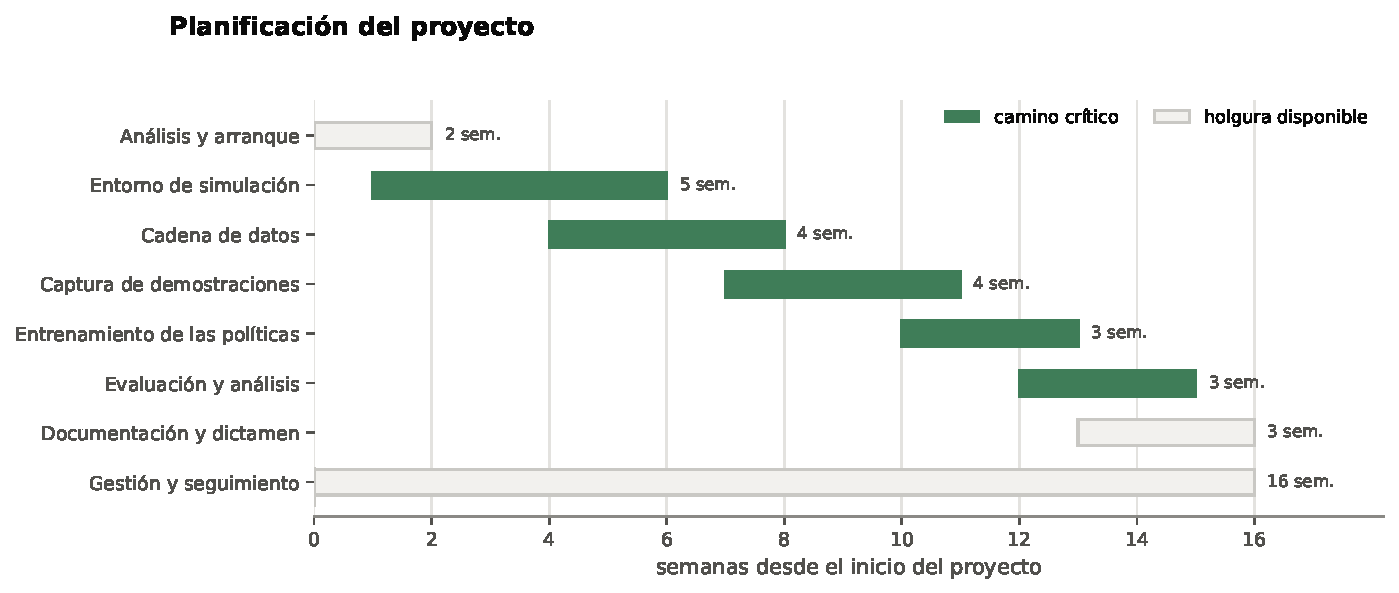
\includegraphics[width=\textwidth]{figuras/sistema/gantt.pdf}
  \caption[Planificación temporal del proyecto]{Planificación temporal del proyecto simulado, con
  indicación del camino crítico}
  \label{fig:gantt}
\end{figure}

El camino crítico —en verde en la figura \ref{fig:gantt}— es la secuencia T1 → T2 → T3 → T4 → T5. No
tiene holgura: un retraso de una semana en el entorno es una semana de retraso en el dictamen. Las
únicas tareas con holgura son las que no están en él: el análisis inicial, que puede comprimirse,
y la documentación, que puede absorber un retraso avanzando en paralelo con la evaluación. La
consecuencia para la gestión es que el esfuerzo de control se concentra en las dos primeras tareas
del camino, donde está la incertidumbre, y no en las últimas, donde el trabajo es predecible.


\section{Gestión de recursos}

\subsection{Especificación de recursos}

\textbf{Recursos humanos.} Cinco perfiles, ninguno a tiempo completo durante todo el proyecto: un
ingeniero de robótica sénior (T0, T1, T6), un técnico de teleoperación (T3), un ingeniero de
aprendizaje automático (T2, T4, y apoyo en T5), un ingeniero de pruebas (T5) y un jefe de proyecto
(T7). El técnico de teleoperación es el recurso más específico: debe ser una sola persona durante
toda la captura, porque el estilo del operador queda grabado en las demostraciones y dos estilos
dan un conjunto de datos peor que uno.

\textbf{Recursos materiales.} La estación de trabajo con sus dos aceleradoras y el visor de realidad
mixta, descritos en la tabla \ref{tab:presupuesto-hardware}, más una red local de baja latencia
entre ambos: la transmisión de vídeo estereoscópico al visor no tolera una red inalámbrica
saturada.

\textbf{Infraestructura.} Un contenedor con la pila de simulación, que aísla sus dependencias y
permite reconstruirlo; almacenamiento para el conjunto de datos y los puntos de control —del orden
de un terabyte—; y un repositorio de control de versiones con los cambios sobre el marco de
terceros conservados como parches.

\subsection{Asignación de recursos}

El cuello de botella es la \textbf{estación de trabajo}, que es única y la necesitan todas las
tareas del camino crítico. La asignación resuelve la contención por dos vías. La primera es la
separación por aceleradora: la GPU 0 queda dedicada a la teleoperación y la grabación durante las
sesiones de captura, porque la transmisión al visor no tolera compartir la GPU, y la GPU 1 corre en
paralelo la aplicación del fondo fotorrealista, los entrenamientos y las evaluaciones. La segunda es
la separación por horario: los trabajos largos y sin supervisión —reproducción de sesiones,
entrenamientos, bloques de cientos de tiradas— se lanzan por la noche, de modo que la máquina
produce veinticuatro horas y las personas la usan de día. Ambas prácticas salen del desarrollo real,
donde una noche de máquina cubrió los seis entrenamientos y las seiscientas tiradas de la curva de
eficiencia.

La carga humana está equilibrada por construcción: los perfiles se suceden a lo largo del camino
crítico —sénior, técnico, aprendizaje automático, pruebas, sénior— y solo el jefe de proyecto
acompaña todo el recorrido. El punto de solapamiento de personas está en las semanas 10 a 13,
cuando captura, entrenamiento y evaluación coinciden, y es donde la máquina, no las personas, marca
el ritmo.


\section{Gestión de riesgos}
\label{sec:riesgos}

\subsection{Identificación de riesgos}

El catálogo de riesgos de la tabla \ref{tab:riesgos} se ha construido a partir de los que
efectivamente se materializaron durante el desarrollo real, más los propios de cualquier proyecto
de esta naturaleza. Es una lista corta a propósito: ocho riesgos que se pueden vigilar valen más
que treinta que nadie revisa.

\begin{table*}[ht]
	\centering
	\caption{Catálogo de riesgos}
	\label{tab:riesgos}
	\makebox[\textwidth]{
		\begin{tabular}{|l|p{5.2cm}|p{7.6cm}|}
			\cline{1-3}
			Id & Riesgo & Causa y efecto \\ \hline
			R1 & Inestabilidad de la pila de realidad mixta & Fallos de configuración sin síntoma visible (transmisión en negro, sobreexposición, cierres al arrancar). Bloquea la captura \\
			R2 & Incompatibilidad entre versiones de bibliotecas & Las bibliotecas de aprendizaje fijan versiones incompatibles con el simulador. Rompe la evaluación o el entrenamiento \\
			R3 & Invalidación de datos ya capturados & Un cambio de decisión o un fallo silencioso del \textit{pipeline} obliga a descartar o regrabar sesiones \\
			R4 & Indisponibilidad de la estación de trabajo & Es única y compartida; una avería o un uso concurrente detiene el camino crítico \\
			R5 & Ampliación no controlada del alcance & Mejoras deseables —fondo fotorrealista, más tareas— desplazan el trabajo comprometido \\
			R6 & Pérdida de cambios sobre el marco de terceros & Modificaciones no versionadas sobre el simulador se destruyen al actualizarlo \\
			R7 & Baja del operador de teleoperación & Es una sola persona; su ausencia detiene la captura y cambiar de operador cambia los datos \\
			R8 & Resultados no concluyentes & La diferencia entre métodos es pequeña y el contraste no la acredita. Debilita el dictamen \\ \hline
		\end{tabular}
	}
\end{table*}

\subsection{Análisis de riesgos}

Cada riesgo se valora en probabilidad e impacto en una escala de uno a cinco, y su exposición es el
producto de ambos. La figura \ref{fig:riesgos} los sitúa en la matriz; la tabla
\ref{tab:analisis-riesgos} recoge la valoración, el plan de mitigación —lo que se hace para que no
ocurra— y el de contingencia —lo que se hace cuando ocurre.

\begin{figure}[htb]
\centering
  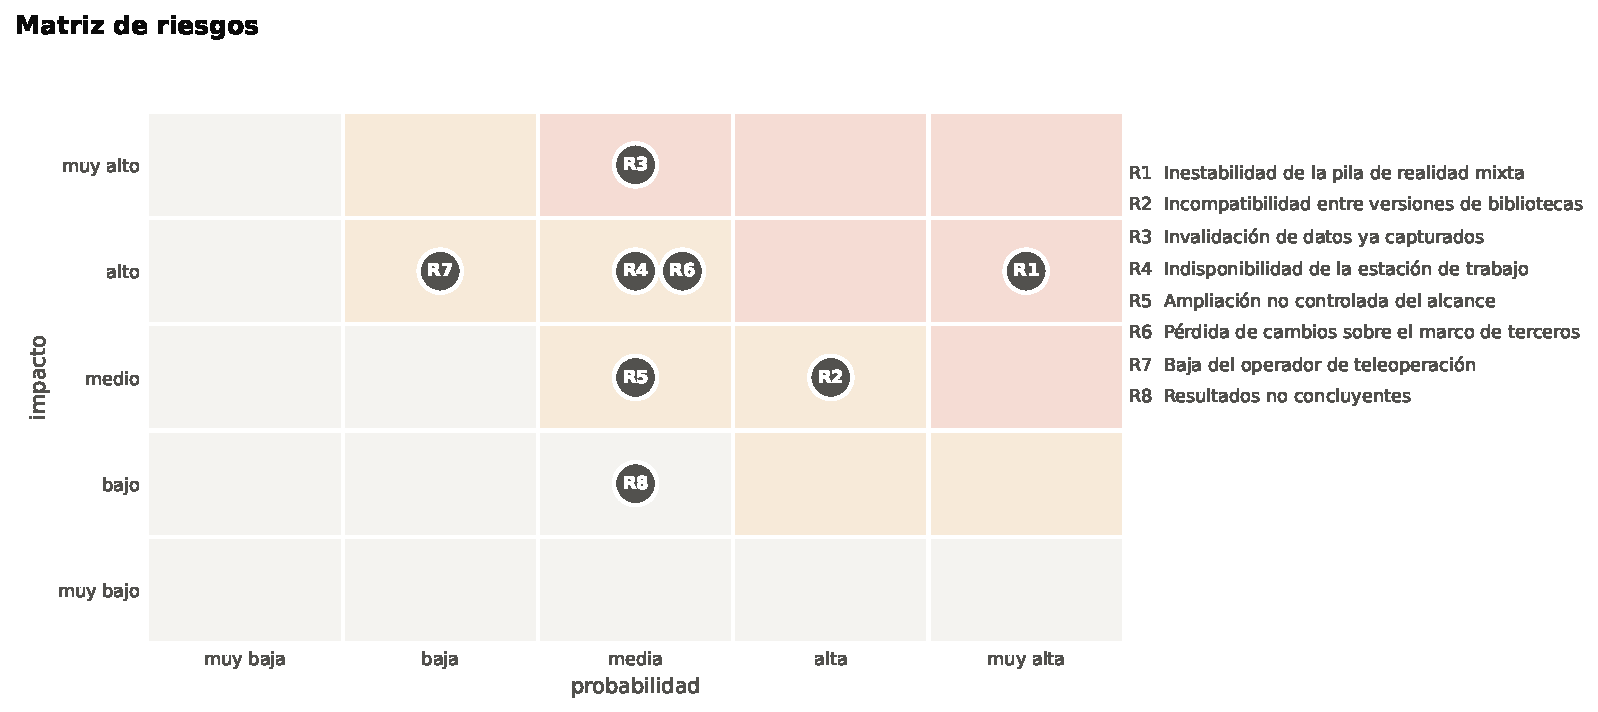
\includegraphics[width=\textwidth]{figuras/sistema/riesgos.pdf}
  \caption[Matriz de riesgos]{Matriz de riesgos del proyecto: probabilidad frente a impacto}
  \label{fig:riesgos}
\end{figure}

\begin{table*}[ht]
	\centering
	\caption{Análisis de riesgos: valoración, mitigación y contingencia}
	\label{tab:analisis-riesgos}
	\makebox[\textwidth]{
		\begin{tabular}{|l|c|c|c|p{5.4cm}|p{5.2cm}|}
			\cline{1-6}
			Id & P & I & P$\times$I & Mitigación & Contingencia \\ \hline
			R1 & 5 & 4 & 20 & Recetas de lanzamiento verificadas y documentadas; tabla de fallos conocidos; monitor en tercera persona para aislar fallos & Semanas de margen en T1; contingencia presupuestaria \\
			R2 & 4 & 3 & 12 & Un entorno de ejecución por método, aislado del simulador; versiones fijadas por escrito & Fijar la última versión compatible y no actualizar \\
			R3 & 3 & 5 & 15 & Verificar una demostración de extremo a extremo antes de grabar en bloque; decisiones de captura cerradas antes del conjunto definitivo & Tratar la sesión perdida como prueba del \textit{pipeline}; regrabar en sesiones de veinticinco \\
			R4 & 3 & 4 & 12 & Reparto por GPU y por horario; trabajos largos desatendidos y reanudables & Reordenar el plan hacia tareas sin máquina (documentación) \\
			R5 & 3 & 3 & 9 & Alcance escrito con exclusiones explícitas; toda ampliación pasa por el jefe de proyecto & Diferir la ampliación a un anexo o a una fase posterior \\
			R6 & 3 & 4 & 12 & Copia versionada de cada cambio como parche; sincronización periódica & Regenerar desde los parches \\
			R7 & 2 & 4 & 8 & Sesiones cortas y frecuentes; documentar el gesto de captura & Reprogramar T3; si se cambia de operador, regrabar el conjunto entero \\
			R8 & 3 & 2 & 6 & Diseño emparejado y tamaño muestral suficiente desde el inicio & Presentar el resultado con su incertidumbre; el dictamen es válido aunque no sea concluyente \\ \hline
		\end{tabular}
	}
\end{table*}

Los dos riesgos que dominan la matriz son R1 y R3, y son también los dos que se materializaron con
más coste en el desarrollo real: la pila de realidad mixta consumió sesiones enteras, y una sesión
de datos completa quedó invalidada por un fallo silencioso del proceso de reproducción antes de
que nadie lo advirtiera. La lección que incorpora el plan es la misma en ambos casos: verificar cada
etapa de extremo a extremo con datos reales antes de invertir esfuerzo en la siguiente, aunque
ello retrase el arranque de la captura. Es más barato perder una semana en T1 que una sesión en T3.
